\chapter{Revue de littérature}
\section{Introduction}
L'intelligence artificielle connaît une évolution rapide. Elle transforme profondément plusieurs domaines technologiques, notamment le traitement automatique des langues naturelles. Grâce aux avancées du \textit{machine learning} et du \textit{deep learning}, les systèmes informatiques sont désormais capables d'analyser, de comprendre et de générer du langage humain, avec une efficacité croissante.

Le \textbf{\ac{TAL}} constitue aujourd'hui un domaine central de l'intelligence artificielle. Parmi ses principales applications figure la traduction automatique. Celle-ci a évolué des approches basées sur des règles vers des modèles neuronaux utilisant les architectures \textbf{Transformer}\footnote{Transformer est un outil d'IA qui traduit des textes en analysant tous les mots d'une phrase en même temps. Cela permet de comprendre le sens général et de proposer une traduction très naturelle } \cite{vaswani2017attention}. Ces modèles offrent des performances élevées, mais nécessitent généralement de grandes quantités de données linguistiques \cite{ranathunga2023neural}.

Les \textbf{\ac{LFR}} demeurent cependant insuffisamment représentées dans les technologies numériques modernes \cite{ranathunga2023neural}. Cette problématique est particulièrement visible dans le contexte africain. De nombreuses langues locales y disposent de peu de corpus numériques et d'outils linguistiques adaptés \cite{agyei2024low}. Le \textbf{ruund} fait partie de ces langues sous-représentées, ce qui limite son intégration dans les systèmes de traduction automatique \cite{haulai2023construction}.

Ce chapitre présente les fondements théoriques liés à l'intelligence artificielle, au \ac{TAL} et à la \textbf{\ac{TAN}}. Il aborde également les problématiques des \ac{LFR}, le contexte linguistique africain ainsi que les travaux existants, afin de justifier l'intérêt scientifique de cette recherche sur la traduction automatique ruund--français.


%------------------------------------------------------------
\section{Méthodologie de la revue de littérature}
%------------------------------------------------------------

\subsubsection{Protocole de recherche documentaire}

Cette revue de littérature a été réalisée selon une démarche systématique, inspirée des recommandations \ac{PRISMA}. Les recherches bibliographiques ont été effectuées dans 4 bases de données scientifiques : Scopus, \ac{ACM}, \ac{IEEE} et Google Scholar.

Les requêtes de recherche ont été construites autour de quatre axes principaux :

\begin{itemize}
    \item la traduction automatique neuronale ;
    \item les langues à faibles ressources ;
    \item la construction et le prétraitement des corpus parallèles ;
    \item les modèles multilingues et les méthodes d'évaluation.
\end{itemize}

Les mots-clés utilisés incluaient notamment \textit{machine translation}, \textit{neural machine translation}, \textit{low-resource languages}, \textit{parallel dataset}, \textit{sentence alignment}, \textit{subword segmentation}, \textit{multilingual models}, \textit{transfer learning}, \textit{Transformer} et \textit{BLEU score}.

La requête de recherche de base, élaborée à partir de ces mots-clés, est présentée ci-dessous. Elle a ensuite été adaptée aux spécificités des différentes bases de données consultées :

\begin{quote}
\texttt{("machine translation" OR "neural machine translation")}\\
\texttt{AND ("low-resource language" OR "under-resourced language")}\\
\texttt{AND ("parallel dataset" OR "dataset construction" OR "sentence alignment" OR "preprocessing")}\\
\texttt{AND ("Transformer" OR "multilingual" OR "transfer learning" OR "evaluation" OR "BLEU")}
\end{quote}


\subsubsection{Critères d'inclusion et d'exclusion}

Les études ont été sélectionnées selon des critères prédéfinis, afin de garantir leur pertinence par rapport aux objectifs de cette recherche. Le Tableau~\ref{tab:criteres_selection} présente l'ensemble des critères appliqués lors du processus de sélection.

\begin{table}[H]
\centering
\renewcommand{\arraystretch}{1.5}
\rowcolors{2}{gray!10}{white}
\begin{tabular}{p{6.8cm}p{6.8cm}}
\toprule
\textbf{Critères d'inclusion} & \textbf{Critères d'exclusion} \\
\midrule
Traduction automatique neuronale pour les langues à faibles ressources & Reconnaissance automatique de la parole (\textit{Speech Recognition}) \\
Construction de corpus parallèles & Classification de textes \\
Alignement de phrases & Analyse de sentiments \\
Prétraitement des données & Recherche d'information (\textit{Information Retrieval}) \\
Segmentation en sous-mots (\ac{BPE}, \ac{SentencePiece}) & Enquêtes (\textit{surveys}) \\
Modèles multilingues & Revues de littérature ou études de synthèse \\
Apprentissage par transfert (\textit{Transfer Learning}) & \\
Métriques d'évaluation telles que \ac{BLEU}, \ac{chrF} & \\
Développement de prototypes de traduction automatique & \\
\bottomrule
\end{tabular}
\caption{Critères d'inclusion et d'exclusion des études sélectionnées}
\label{tab:criteres_selection}
\end{table}

\subsubsection{Processus de sélection des études}

La sélection des publications a été réalisée en plusieurs étapes. Les doublons ont d'abord été supprimés, après l'identification initiale des documents dans les différentes bases de données. Les titres et résumés ont ensuite été examinés, afin d'évaluer leur pertinence au regard des critères d'inclusion et d'exclusion. Les articles retenus ont finalement fait l'objet d'une lecture intégrale, avant leur inclusion dans l'analyse finale.

Le processus complet de sélection des études est présenté dans le diagramme \ac{PRISMA} ci-dessous.

\begin{figure}[H]
    \centering
    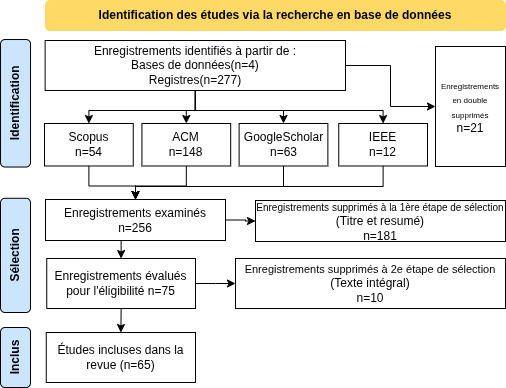
\includegraphics[width=0.85\textwidth]{Images/prisma_diagram.png}
    \caption{Diagramme PRISMA du processus de sélection des études \cite{Page2021PRISMA}}
    \label{fig:prisma}
\end{figure}


%------------------------------------------------------------
\section{Fondements théoriques}
%------------------------------------------------------------

\subsection{Intelligence artificielle}

\subsubsection{Définition et évolution de l'intelligence artificielle}

L'\textbf{\ac{IA}} désigne un ensemble de méthodes et de techniques permettant à une machine de reproduire certaines capacités cognitives humaines, telles que l'apprentissage, le raisonnement, la résolution de problèmes ou la prise de décision. Ce domaine de recherche vise principalement à concevoir des systèmes capables d'exécuter automatiquement des tâches nécessitant normalement l'intelligence humaine \cite{Goodfellow-et-al-2016}.

L'évolution des capacités de calcul, la disponibilité massive des données numériques ainsi que les progrès des réseaux de neurones ont favorisé l'émergence du \textit{machine learning}, puis du \textit{deep learning} \cite{Goodfellow-et-al-2016}. Ces approches permettent aux systèmes informatiques d'apprendre automatiquement des représentations complexes à partir des données. Elles améliorent ainsi considérablement les performances dans plusieurs domaines, tels que la vision par ordinateur, la reconnaissance vocale et le traitement automatique des langues \cite{ranathunga2023neural}.

\subsubsection{\ac{IA} et traitement automatique des langues}

Le \ac{TAL} applique les méthodes de l'\ac{IA} au langage humain : l'analyse, la compréhension et la génération de texte par les machines. Cette branche combine des connaissances issues de l'informatique, de la linguistique et de l'apprentissage automatique \cite{ranathunga2023neural}. Une définition plus détaillée de ce domaine, ainsi que de ses principales applications, est proposée en section~\ref{sec:tal-def}.

Les progrès récents du \textit{deep learning} et des architectures \textbf{Transformer} ont considérablement amélioré les performances des systèmes \ac{NLP}, en particulier dans les tâches de \textbf{TAN (\ac{NMT})} \cite{vaswani2017attention, ranathunga2023neural, agyei2025dynamic}.

%------------------------------------------------------------
\subsection{Machine Learning}
%------------------------------------------------------------

\subsubsection{Définition du Machine Learning}

Le \ac{ML} constitue une branche de l'intelligence artificielle. Il permet aux systèmes informatiques d'apprendre automatiquement à partir des données, sans être explicitement programmés pour chaque tâche \cite{Goodfellow-et-al-2016}. Son objectif principal est de construire des modèles capables d'identifier des relations, des régularités ou des représentations à partir des données, afin d'effectuer des prédictions ou des décisions automatiques \cite{Goodfellow-et-al-2016}.

\subsubsection{Types d'apprentissage}

Le \ac{ML} regroupe principalement trois grandes catégories d'apprentissage : l'apprentissage supervisé, l'apprentissage non supervisé et l'apprentissage par renforcement \cite{Goodfellow-et-al-2016}.

\paragraph{L'Apprentissage supervisé :}

repose sur l'utilisation de données annotées, contenant des exemples d'entrée et de sortie. Le modèle apprend alors à établir une relation entre les données d'entrée et les résultats attendus, afin de prédire correctement de nouvelles données \cite{Goodfellow-et-al-2016}. Cette approche est largement utilisée dans les tâches de classification, de régression et de traduction automatique \cite{ranathunga2023neural}.

\subsubsection{Apprentissage supervisé dans la traduction automatique}

La \textbf{traduction automatique neuronale} (\ac{TAN}) repose principalement sur l'apprentissage supervisé. Dans cette approche, le modèle est entraîné à partir de \textbf{corpus parallèles}, contenant des phrases dans une langue source et leurs traductions correspondantes dans une langue cible \cite{ranathunga2023neural, haulai2023construction, jindal2017building}.

%------------------------------------------------------------
\subsection{Deep Learning}
%------------------------------------------------------------

\subsubsection{Réseaux de neurones artificiels}

Les \textbf{\ac{RNA}} sont des modèles informatiques inspirés du fonctionnement biologique du cerveau humain \cite{Goodfellow-et-al-2016}. Ils sont composés d'unités appelées \textbf{neurones artificiels}, organisées en différentes couches interconnectées. Chaque neurone reçoit des données en entrée, effectue des calculs mathématiques, puis transmet un résultat à la couche suivante \cite{Goodfellow-et-al-2016}.

\subsubsection{Réseaux neuronaux profonds}

Le \textbf{\textit{\ac{DL}}} correspond à une évolution des réseaux de neurones artificiels, utilisant plusieurs couches cachées. Ces architectures profondes permettent d'apprendre des représentations hiérarchiques et complexes des données. Elles améliorent ainsi considérablement les performances des modèles d'intelligence artificielle \cite{Goodfellow-et-al-2016}.

Les réseaux neuronaux profonds ont connu un développement important, grâce à l'augmentation de la puissance de calcul, à la disponibilité des données massives et aux progrès des processeurs graphiques \cite{Goodfellow-et-al-2016}. Ils sont aujourd'hui utilisés dans plusieurs domaines, tels que la vision par ordinateur, la reconnaissance vocale et le traitement automatique des langues \cite{ranathunga2023neural}.

\subsubsection{Importance du Deep Learning dans le \ac{NLP}}

Le \ac{DL} a profondément transformé le traitement automatique des langues naturelles. Contrairement aux approches traditionnelles, basées sur des règles linguistiques ou des caractéristiques manuellement définies, les modèles profonds apprennent automatiquement les représentations linguistiques à partir des données \cite{Goodfellow-et-al-2016, ranathunga2023neural}.

Cette évolution a permis l'apparition de modèles neuronaux performants, capables de traiter des tâches complexes telles que la \textbf{\ac{TA}}, la génération de texte, les agents conversationnels et l'analyse sémantique \cite{ranathunga2023neural, agyei2025dynamic}. Les architectures modernes comme les \textbf{Transformers} ont particulièrement amélioré la qualité des systèmes \ac{NLP}, en facilitant la prise en compte du contexte linguistique \cite{vaswani2017attention}.

%------------------------------------------------------------
\subsection{Traitement automatique des langues naturelles}
\label{sec:tal-def}
%------------------------------------------------------------

\subsubsection{Définition du \ac{TAL}}

Le traitement automatique des langues naturelles (\textit{Natural Language Processing}, \ac{NLP}) est la branche de l'intelligence artificielle consacrée à l'analyse, à la compréhension et à la génération automatique du langage humain par les machines. Comme indiqué en introduction de ce chapitre, ce domaine associe informatique, linguistique et apprentissage automatique \cite{ranathunga2023neural}.

Le \ac{TAL} vise principalement à faciliter l'interaction entre l'homme et la machine, à travers le traitement des données textuelles et vocales. Les avancées récentes du \ac{DL} ont fortement amélioré les capacités des systèmes \ac{NLP} dans plusieurs tâches linguistiques complexes \cite{vaswani2017attention}.

\subsubsection{Principales applications du \ac{TAL}}

Le \ac{TAL} possède de nombreuses applications dans les technologies numériques modernes. Outre la traduction automatique, déjà évoquée, ses usages recouvrent la reconnaissance vocale, les assistants conversationnels, l'analyse de sentiments ainsi que les systèmes de recherche d'information \cite{ranathunga2023neural}.

\subsubsection{\ac{TAL} et langues africaines}

Malgré les progrès importants du \ac{TAL}, plusieurs langues africaines demeurent faiblement représentées dans les ressources numériques et les systèmes \ac{NLP} modernes. Cette situation s'explique notamment par le manque de corpus numériques, l'absence de standardisation linguistique et la rareté des outils de traitement adaptés \cite{agyei2024low}.

Les \textbf{langues africaines à faibles ressources} rencontrent ainsi des difficultés importantes dans le développement d'applications telles que la \textbf{traduction automatique neuronale}. Le manque de données parallèles limite l'entraînement efficace des modèles de \ac{DL}, ce qui réduit les performances des systèmes développés pour ces langues \cite{mandiya2026lingala}.

%------------------------------------------------------------
\subsection{Traduction automatique}
%------------------------------------------------------------

\subsubsection{Définition de la traduction automatique}

La \textbf{traduction automatique} (\ac{TA}) désigne l'utilisation de systèmes informatiques capables de traduire automatiquement un texte d'une langue source vers une langue cible, sans intervention humaine directe. Elle constitue l'une des principales applications du traitement automatique des langues naturelles \cite{ranathunga2023neural}.

L'objectif de la \ac{TA} est de produire des traductions grammaticalement correctes et sémantiquement cohérentes, tout en conservant le sens du texte original. Les performances des systèmes de traduction ont considérablement évolué, grâce aux progrès du \ac{ML} et du \ac{DL} \cite{vaswani2017attention}.

\subsubsection{\ac{TAB}}

Les premiers systèmes de traduction automatique reposaient principalement sur des approches basées sur des règles linguistiques (\textit{\ac{RBMT}}). Ces systèmes utilisaient des dictionnaires bilingues ainsi que des règles grammaticales définies manuellement par des experts linguistes \cite{ranathunga2023neural}.

Cette approche nécessitait une importante expertise linguistique et un travail manuel considérable pour chaque paire de langues. Elle permettait un certain contrôle linguistique, mais présentait des difficultés importantes face aux ambiguïtés lexicales et aux variations contextuelles des langues naturelles \cite{dundjer2020automatic}.

\subsubsection{\ac{TAS}}

La \textbf{\ac{TAS}} (\textit{\ac{SMT}}) a ensuite remplacé progressivement les approches basées sur des règles. Cette méthode repose sur l'apprentissage de relations statistiques, à partir de grands corpus parallèles contenant des phrases alignées dans plusieurs langues.

Les systèmes statistiques analysent les probabilités de correspondance entre les mots et les segments linguistiques, afin de générer des traductions automatiques. Cette approche a permis d'améliorer significativement la qualité des traductions, par rapport aux systèmes basés uniquement sur des règles linguistiques \cite{ahmadnia2018neural}.

\subsubsection{Limites des approches classiques}

Les approches classiques de traduction automatique présentent plusieurs limites, malgré leurs contributions importantes. Les systèmes à base de règles exigent un travail manuel conséquent et s'adaptent mal à de nouvelles langues, tandis que les approches statistiques restent tributaires de grands corpus parallèles et gèrent difficilement le contexte global des phrases \cite{ranathunga2023neural}.

Ces limitations ont favorisé l'émergence de la \textbf{traduction automatique neuronale} (\ac{TAN}). Celle-ci est capable d'apprendre automatiquement des représentations linguistiques plus complexes, et de produire des traductions plus naturelles et plus cohérentes \cite{vaswani2017attention}.

Le Tableau~\ref{tab:comparaison_ta} présente une synthèse comparative des trois grandes approches de traduction automatique, selon plusieurs critères pertinents.

\begin{table}[H]
\centering
\renewcommand{\arraystretch}{1.5}
\rowcolors{2}{gray!10}{white}
\begin{tabular}{p{3.2cm}p{3.5cm}p{3.5cm}p{3.5cm}}
\toprule
\textbf{Critère} & \textbf{\ac{RBMT}} & \textbf{\ac{SMT}} & \textbf{\ac{NMT}} \\
\midrule
\textbf{Période} & Années 1950--1990 & Années 1990--2015 & Depuis 2015 \\
\textbf{Principe} & Règles linguistiques et dictionnaires bilingues définis manuellement & Modèles probabilistes appris à partir de corpus parallèles & Réseaux de neurones profonds entraînés sur corpus parallèles \\
\textbf{Données requises} & Règles et lexiques manuels & Grands corpus parallèles & Grands corpus parallèles \\
\textbf{Apprentissage} & Non automatique & Automatique (statistique) & Automatique (neuronal) \\
\textbf{Gestion du contexte} & Limitée & Partielle (n-grammes) & Globale (mécanisme d'attention) \\
\textbf{Qualité des traductions} & Contrôlée mais rigide & Meilleure que \ac{RBMT} & Meilleure qualité globale \\
\textbf{Langues à faibles ressources} & Difficile (expertise manuelle) & Difficile (manque de corpus) & Difficile (manque de données) \\
\textbf{Exemples de systèmes} & Systran, Apertium & Moses, Pharaoh & mBART, NLLB... \\
\bottomrule
\end{tabular}
\caption{Comparaison des approches de traduction automatique}
\label{tab:comparaison_ta}
\end{table}

%------------------------------------------------------------
\subsection{Traduction automatique neuronale}
%------------------------------------------------------------

\subsubsection{Principe de la traduction neuronale}

La \textbf{traduction automatique neuronale} (\textit{\ac{NMT}}) constitue une approche moderne de traduction automatique, fondée sur les réseaux de neurones profonds. Contrairement aux approches classiques basées sur des règles ou des probabilités statistiques, la traduction neuronale apprend automatiquement les relations linguistiques entre les langues à partir de corpus parallèles \cite{ranathunga2023neural}.

Le modèle reçoit une phrase dans une langue source et génère directement sa traduction dans une langue cible. Cette approche permet de produire des traductions plus fluides, plus cohérentes et mieux adaptées au contexte linguistique \cite{vaswani2017attention}.

\subsubsection{Architectures encodeur-décodeur}

Les premiers systèmes de traduction neuronale reposaient principalement sur l'architecture \textbf{encodeur-décodeur} (\textit{Encoder--Decoder}). Dans cette architecture, l'encodeur transforme la phrase source en une représentation numérique, appelée \textbf{vecteur de contexte}. Le décodeur utilise ensuite cette représentation pour générer progressivement la phrase traduite \cite{ranathunga2023neural}.

Cette architecture a permis d'améliorer considérablement les performances de la traduction automatique, en facilitant l'apprentissage des relations sémantiques entre les langues \cite{lalrempuii2021improved}.

La Figure~\ref{fig:encoder_decoder} illustre le fonctionnement de l'architecture encodeur-décodeur utilisée dans les premiers systèmes de traduction neuronale.

\begin{figure}[H]
    \centering
    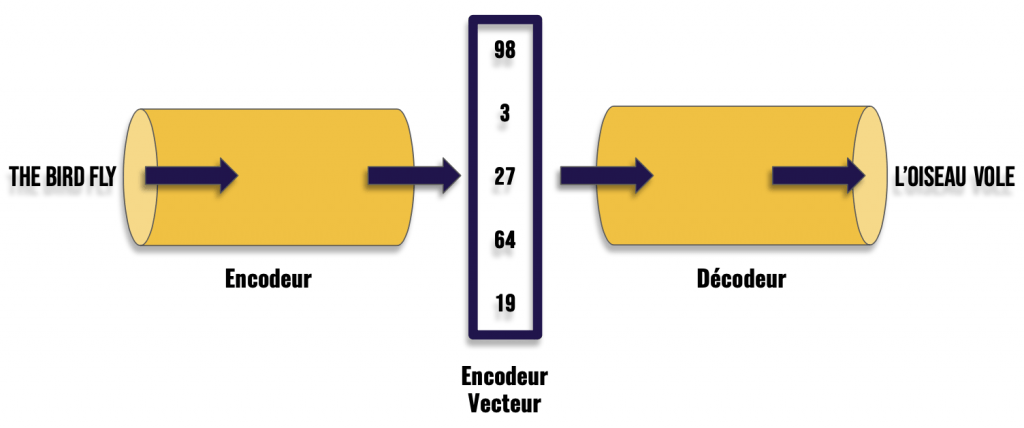
\includegraphics[width=0.75\textwidth]{Images/encode_decoder.png}
    \caption[L’Encodeur-Décodeur]{L’Encodeur-Décodeur \cite{keldenich2021encoder}}
    \label{fig:encoder_decoder}
\end{figure}

\subsubsection{Mécanisme d'attention}

Le \textbf{mécanisme d'attention} (\textit{Attention Mechanism}) a été introduit afin de résoudre certaines limites des architectures encodeur-décodeur classiques, notamment les difficultés liées aux longues phrases \cite{vaswani2017attention}.

L'attention permet au modèle de se concentrer sur les parties les plus pertinentes de la phrase source, lors de la génération de chaque mot traduit. Cette approche améliore la prise en compte du contexte linguistique. Elle augmente ainsi la qualité des traductions produites \cite{gangar2021hindi}.

Le mécanisme d'attention constitue également la base des architectures \textbf{Transformer} utilisées dans les modèles modernes de traduction automatique neuronale \cite{vaswani2017attention}.

\subsubsection{Avantages des approches neuronales}

Les approches neuronales présentent plusieurs avantages par rapport aux méthodes classiques de traduction automatique. Elles permettent de produire des traductions plus naturelles, plus cohérentes et mieux contextualisées. Elles réduisent également la nécessité de définir manuellement des règles linguistiques complexes \cite{ranathunga2023neural}.

Les modèles neuronaux sont capables d'apprendre automatiquement des représentations linguistiques riches. Ils gèrent aussi mieux les relations contextuelles entre les mots. Leurs performances dépendent cependant fortement de la disponibilité des données d'entraînement et des ressources de calcul. Ce constat représente un défi important pour les \textbf{langues à faibles ressources (\ac{LFR})} telles que le ruund \cite{haulai2023construction}.

%------------------------------------------------------------
\subsection{Architectures Transformer}
%------------------------------------------------------------

\subsubsection{Origine des Transformers}

Les architectures Transformer\footnote{\url{https://poloclub.github.io/transformer-explainer/}} ont été introduites en 2017, afin d'améliorer les performances des modèles de traitement automatique des langues. Contrairement aux réseaux récurrents traditionnels (\ac{RNN}), les Transformers reposent principalement sur le mécanisme d'attention. Ce choix architectural permet un traitement parallèle des données textuelles \cite{vaswani2017attention}.

Cette architecture a marqué une évolution majeure dans le domaine du \ac{NLP}, en améliorant la qualité des tâches linguistiques telles que la traduction automatique, la génération de texte et la compréhension du langage naturel \cite{ranathunga2023neural}.

\subsubsection{Fonctionnement du mécanisme d'attention}

Le \textbf{mécanisme d'attention} permet au modèle d'identifier les éléments les plus importants d'une phrase, lors du traitement linguistique. Pour chaque mot, le système évalue les relations avec les autres mots de la séquence, afin de mieux comprendre le contexte global \cite{vaswani2017attention}.

Cette approche améliore la gestion des dépendances linguistiques longues. Elle réduit ainsi certaines limitations des architectures récurrentes classiques. Les Transformers utilisent principalement une variante appelée \textbf{\textit{Self-Attention}}, dans laquelle chaque mot peut interagir directement avec les autres mots de la phrase \cite{vaswani2017attention}.

La Figure~\ref{fig:architecture_transformer} illustre l'architecture générale du modèle Transformer, telle que proposée par \citeauthor{vaswani2017attention}.

\begin{figure}[H]
    \centering
    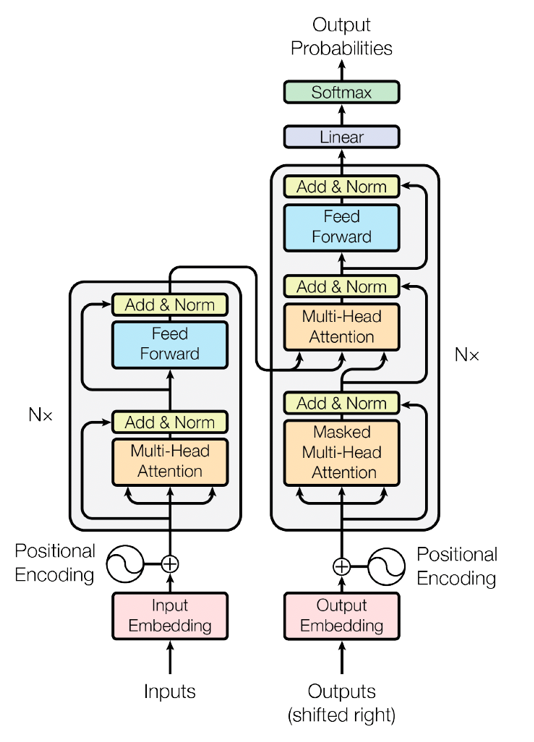
\includegraphics[width=0.75\textwidth]{Images/Archi-transformers.png}
    \caption[Architecture Transformer]{Architecture Transformer \cite{vaswani2017attention}}
    \label{fig:architecture_transformer}
\end{figure}

\subsubsection{Représentation contextuelle des mots}

Les architectures Transformer permettent de générer des \textbf{représentations contextuelles} des mots. Contrairement aux représentations statiques traditionnelles, le sens d'un mot est interprété selon son contexte dans la phrase \cite{vaswani2017attention}.

Cette capacité améliore considérablement la compréhension sémantique. Elle réduit aussi les ambiguïtés linguistiques. Les modèles modernes peuvent ainsi produire des traductions plus cohérentes et mieux adaptées au contexte du texte source \cite{kozhirbayev2024enhancing}.

\subsubsection{Transformers et traduction multilingue}

Les Transformers constituent aujourd'hui la base des principaux modèles de traduction automatique multilingue, tels que \textbf{mBART}, \textbf{MarianMT} ou \textbf{NLLB}. Ces modèles sont capables d'apprendre simultanément plusieurs langues, à partir de grands corpus multilingues \cite{kozhirbayev2024enhancing}.

Cette approche facilite le transfert de connaissances entre les langues à fortes ressources et les \textbf{langues à faibles ressources}. Elle représente ainsi une solution importante pour le développement de systèmes de traduction automatique adaptés aux langues africaines peu représentées numériquement, notamment le ruund \cite{mandiya2026lingala}.

%------------------------------------------------------------
\subsection{Modèles multilingues de traduction}
%------------------------------------------------------------

\subsubsection{Modèles pré-entraînés multilingues}

Les \textbf{modèles pré-entraînés multilingues} sont des modèles neuronaux entraînés sur de grandes quantités de données, provenant de plusieurs langues simultanément. Leur objectif est d'apprendre des représentations linguistiques générales, capables d'être réutilisées dans différentes tâches de traitement automatique des langues, notamment la traduction automatique \cite{ranathunga2023neural}.

Ces modèles reposent principalement sur les architectures \textbf{Transformer} et exploitent le transfert de connaissances entre langues. Cette approche est particulièrement importante pour les \textbf{langues à faibles ressources}, car elle permet d'améliorer les performances, même lorsque les données disponibles sont limitées \cite{nguyen2017transfer}.

\subsubsection{Présentation de \ac{mBART}}

\textbf{mBART-50} est un modèle multilingue de traduction automatique, fondé sur l'architecture Transformer. Il repose sur une stratégie de pré-entraînement séquence-à-séquence, permettant au modèle d'apprendre des représentations linguistiques à partir de plusieurs langues \cite{kozhirbayev2024enhancing}.

Le modèle prend en charge plusieurs dizaines de langues et peut être adapté à des tâches spécifiques grâce au \textit{fine-tuning}. mBART-50 est particulièrement utilisé dans les contextes multilingues et les langues à faibles ressources, grâce à sa capacité de transfert linguistique \cite{kozhirbayev2024enhancing}.

\subsubsection{Présentation de NLLB-200-distilled-600M}

\textbf{NLLB-200-distilled-600M} est un modèle développé dans le cadre du projet \textit{\ac{NLLB}}. Son objectif principal est d'améliorer la traduction automatique pour les langues sous-représentées dans les technologies numériques \cite{ranathunga2023neural}.

Ce modèle prend en charge un très grand nombre de langues, notamment plusieurs langues africaines. Grâce à son entraînement multilingue massif, il offre de bonnes capacités de généralisation et de transfert vers les langues à faibles ressources. La version distillée permet également de réduire les besoins en ressources computationnelles, tout en conservant des performances importantes \cite{agyei2025dynamic}.

\subsubsection{Présentation de \ac{MarianMT}}

\textbf{\ac{MarianMT}} est un modèle de traduction automatique neuronale, basé sur l'architecture Transformer et développé pour les tâches de traduction multilingue. Il est largement utilisé dans les bibliothèques \ac{NLP} modernes, grâce à sa flexibilité et à sa compatibilité avec plusieurs paires de langues \cite{angel2023comparing}.

MarianMT propose des modèles pré-entraînés spécialisés pour différentes combinaisons linguistiques. Il peut également être adapté à des contextes spécifiques à travers le \textit{fine-tuning} \cite{lalrempuii2023investigating}.

\subsubsection{Comparaison générale des modèles}

Les modèles mBART-50, NLLB-200-distilled-600M et MarianMT reposent tous sur les architectures Transformer. Ils utilisent tous des approches multilingues de traduction automatique neuronale. Le Tableau~\ref{tab:comparaison_modeles} présente une synthèse comparative de ces trois modèles, selon plusieurs critères pertinents pour le contexte des langues à faibles ressources \cite{kozhirbayev2024enhancing, ranathunga2023neural}.


\begin{table}[H]
\centering

\renewcommand{\arraystretch}{1.5}
\rowcolors{2}{gray!10}{white}
\begin{tabular}{p{3.2cm}p{3.4cm}p{3.4cm}p{3.4cm}}
\toprule
\textbf{Critère} & \textbf{\ac{mBART}-50} & \textbf{\ac{NLLB}-200-distilled-600M} & \textbf{\ac{MarianMT}} \\
\midrule
\textbf{Architecture} & Transformer seq2seq & Transformer seq2seq & Transformer seq2seq \\
\textbf{Nombre de langues} & 50 langues & 200+ langues & Paires spécifiques \\
\textbf{Stratégie de pré-entraînement} & Débruitage multilingue & Entraînement supervisé massif & Entraînement supervisé par paire \\
\textbf{Langues africaines} & Couverture limitée & Couverture étendue & Très limitée \\
\textbf{Adaptation (fine-tuning)} & Oui & Oui & Oui \\
\textbf{Ressources computationnelles} & Modérées & Réduites (version distillée) & Légères \\
\textbf{Langues à faibles ressources} & Performant après fine-tuning & Orienté LFR & Dépend de la paire \\
\textbf{Disponibilité} & HuggingFace & HuggingFace & HuggingFace \\
\bottomrule
\end{tabular}
\caption{Comparaison des modèles multilingues de traduction automatique}
\label{tab:comparaison_modeles}
\end{table}

Le choix du modèle dépend principalement de plusieurs facteurs, tels que la disponibilité des données, les ressources computationnelles et les objectifs de la tâche de traduction \cite{ranathunga2023neural}.

%------------------------------------------------------------
\subsection{Entraînement et adaptation des modèles neuronaux}
%------------------------------------------------------------

\subsubsection{Pré-entraînement des modèles}

Le \textbf{pré-entraînement} consiste à entraîner un modèle neuronal sur de très grandes quantités de données textuelles, avant son utilisation dans une tâche spécifique. Cette étape permet au modèle d'apprendre des représentations linguistiques générales, telles que les relations syntaxiques, sémantiques et contextuelles entre les mots \cite{Goodfellow-et-al-2016, ranathunga2023neural}.

\subsubsection{Fine-tuning des modèles multilingues}

Le \textbf{\textit{fine-tuning}} correspond à l'adaptation d'un modèle pré-entraîné à une tâche particulière, à l'aide d'un corpus spécialisé. Dans le contexte de la traduction automatique, cette étape consiste à réentraîner le modèle sur des données parallèles spécifiques à une paire de langues donnée \cite{kozhirbayev2024enhancing}.

Le \textit{fine-tuning} permet d'améliorer les performances du modèle dans un domaine précis, tout en exploitant les connaissances acquises lors du pré-entraînement. Cette méthode est particulièrement utilisée pour les \textbf{langues à faibles ressources}, car elle réduit les besoins en grandes quantités de données d'entraînement \cite{ma2025dongba}.

\subsubsection{Transfer learning dans les langues à faibles ressources}

Le \textbf{\textit{Transfer Learning}}, ou \textbf{apprentissage par transfert}, consiste à réutiliser les connaissances acquises par un modèle sur des langues ou des tâches disposant de grandes quantités de données, afin d'améliorer les performances sur des langues moins représentées \cite{nguyen2017transfer, lalrempuii2023investigating}.

\subsubsection{Paramètres et poids des modèles}

Les modèles neuronaux sont composés de nombreux paramètres, appelés \textbf{poids} (\textit{weights}), appris automatiquement pendant l'entraînement. Ces paramètres représentent les relations mathématiques apprises par le modèle à partir des données \cite{Goodfellow-et-al-2016}.

Les grands modèles multilingues possèdent souvent des millions, voire des milliards de paramètres. L'ajustement de ces poids, pendant l'entraînement et le \textit{fine-tuning}, permet au système d'améliorer progressivement ses performances de traduction \cite{kozhirbayev2024enhancing}.

L'augmentation du nombre de paramètres entraîne cependant aussi des besoins plus importants en mémoire, en puissance de calcul et en données d'entraînement. Cette contrainte représente un défi majeur dans les contextes de \textbf{langues à faibles ressources (\ac{LFR})} et d'environnements computationnels limités \cite{agyei2025dynamic}.
%------------------------------------------------------------
\subsubsection{Hyperparamètres d'entraînement}

Les performances des modèles neuronaux dépendent fortement du choix des \textbf{hyperparamètres d'entraînement}. Contrairement aux paramètres appris automatiquement par le modèle, les hyperparamètres sont définis avant l'entraînement et influencent directement la qualité de l'apprentissage \cite{Goodfellow-et-al-2016}. Les principaux hyperparamètres utilisés dans les systèmes de \ac{TAN} sont les suivants :

\begin{itemize}

    \item Le \textbf{\textit{learning rate}} détermine la vitesse de mise à jour des poids du modèle pendant l'apprentissage. Une valeur trop élevée peut entraîner une instabilité de l'entraînement. Une valeur trop faible peut, à l'inverse, ralentir la convergence du modèle.

    \item Le \textbf{\textit{batch size}} correspond au nombre d'exemples traités simultanément lors d'une étape d'entraînement. Une taille de batch élevée améliore généralement la stabilité des calculs, mais nécessite davantage de mémoire.

    \item Les \textbf{\textit{epochs}} représentent le nombre de passages complets du modèle sur l'ensemble des données d'entraînement. Un nombre insuffisant d'epochs peut produire un sous-apprentissage (\textit{underfitting}). Un nombre trop élevé peut, à l'inverse, provoquer un surapprentissage (\textit{overfitting}).

\end{itemize}

Le choix approprié de ces hyperparamètres est déterminant pour la convergence et les performances finales du modèle. Ce choix est particulièrement sensible dans les contextes à faibles ressources, où les données d'entraînement sont limitées \cite{kozhirbayev2024enhancing}.

%------------------------------------------------------------
\subsubsection{Contraintes computationnelles}

L'entraînement des modèles neuronaux de traduction automatique nécessite des ressources computationnelles importantes. Les contraintes computationnelles concernent principalement l'utilisation des \textbf{\ac{GPU}}, la capacité de stockage des données ainsi que le temps nécessaire pour entraîner et ajuster les modèles. Ces contraintes deviennent encore plus importantes dans les contextes de recherche disposant de ressources matérielles limitées \cite{Goodfellow-et-al-2016}.

Dans le cadre des \textbf{langues à faibles ressources}, les difficultés computationnelles s'ajoutent souvent aux limitations liées aux données linguistiques. Il devient alors nécessaire d'utiliser des approches adaptées, telles que le \textit{fine-tuning} de modèles pré-entraînés, les modèles distillés ou les architectures optimisées, afin de réduire les coûts computationnels tout en maintenant des performances satisfaisantes \cite{agyei2025dynamic}.

%------------------------------------------------------------
\subsection{Tokenisation et représentations linguistiques}
%------------------------------------------------------------

\subsubsection{Tokenisation des textes}

La \textbf{tokenisation} consiste à découper un texte en unités élémentaires appelées \textbf{tokens}. Ces unités peuvent correspondre à des mots, des caractères ou des sous-mots, selon l'approche utilisée. Cette étape constitue une phase essentielle du prétraitement des données dans les systèmes de \ac{TAL} \cite{ranathunga2023neural}.

La tokenisation permet de transformer les textes bruts en représentations exploitables par les modèles neuronaux \cite{Goodfellow-et-al-2016}.

\subsubsection{Segmentation en sous-mots}

Les modèles modernes de traduction automatique utilisent généralement une \textbf{segmentation en sous-mots}, plutôt qu'une simple segmentation par mots entiers. Cette approche consiste à découper les mots en unités linguistiques plus petites, afin de mieux gérer les mots rares ou inconnus \cite{toraman2022impact}.

Cette stratégie est particulièrement adaptée aux langues morphologiquement riches et agglutinantes. Pour ces langues, une tokenisation par mots entiers produirait un vocabulaire très large et peu généralisable \cite{chen-fazio-2021-morphologically}.

\subsubsection{SentencePiece}

\textbf{\ac{SentencePiece}} est une méthode de tokenisation largement utilisée dans les modèles Transformer modernes. Contrairement aux approches traditionnelles, dépendantes des espaces entre les mots, SentencePiece traite directement le texte brut. Il apprend ainsi automatiquement les unités de segmentation les plus pertinentes \cite{meyer2024systematic}.

\subsubsection{Embeddings multilingues}

Les \textbf{embeddings multilingues} sont des représentations vectorielles, qui projettent les mots de plusieurs langues dans un même espace sémantique. Les mots ayant des significations proches possèdent ainsi des représentations vectorielles similaires \cite{ali2026hybrid, meyer2024systematic}.

\subsubsection{Problème des mots hors vocabulaire (OOV)}

Les \textbf{mots hors vocabulaire} (\textit{\ac{OOV}}) correspondent aux mots absents du vocabulaire appris par le modèle pendant l'entraînement. Ce problème est fréquent dans les langues à faibles ressources, en raison du manque de données disponibles \cite{ranathunga2023neural, toraman2022impact}.

%------------------------------------------------------------
\subsection{Corpus parallèles}
%------------------------------------------------------------

\subsubsection{Définition d'un corpus parallèle}

Un \textbf{corpus parallèle} est un ensemble de textes alignés dans au moins deux langues différentes. Chaque phrase de la langue source possède une traduction correspondante dans la langue cible. Les corpus constituent une ressource fondamentale dans les systèmes de traduction automatique neuronale \cite{ranathunga2023neural, haulai2023construction}.

\subsubsection{Importance des corpus dans la traduction automatique}

Les modèles de traduction automatique apprennent les relations linguistiques à partir des corpus parallèles. La qualité, la taille et la diversité des données influencent directement les performances des systèmes neuronaux \cite{ranathunga2023neural, agyei2024low}.

\subsubsection{Méthodes de collecte des données}

La collecte des données peut être réalisée à partir de plusieurs sources, telles que les documents bilingues, les textes religieux, les contenus éducatifs, les traductions manuelles ou les ressources communautaires \cite{haulai2023construction, jindal2017building}.

Dans le contexte des \textbf{langues africaines à faibles ressources}, la collecte des données nécessite souvent un travail manuel important, en raison du manque de ressources numériques disponibles \cite{agyei2024low, mandiya2026lingala}.

\subsubsection{Nettoyage et normalisation}

Le \textbf{nettoyage} des données consiste à supprimer les erreurs, les doublons et les phrases mal alignées présentes dans le corpus. La \textbf{normalisation} permet quant à elle d'uniformiser les textes, afin de faciliter l'apprentissage du modèle \cite{sharma2023fully}.

Cette étape peut inclure la conversion en minuscules, la suppression des caractères inutiles ainsi que la correction de certaines incohérences orthographiques \cite{ali2026hybrid}.

\subsubsection{Alignement des phrases}

L'\textbf{alignement} consiste à associer correctement chaque phrase de la langue source avec sa traduction dans la langue cible. Cette étape est essentielle pour garantir la qualité des données utilisées pendant l'entraînement des modèles neuronaux \cite{ali2026hybrid, haulai2023construction}.

\subsubsection{Corpus religieux et poétiques dans les langues à faibles ressources}

Pour de nombreuses \textbf{langues à faibles ressources}, les textes religieux et poétiques constituent les piliers fondamentaux pour la construction des premiers corpus parallèles, en raison de leur disponibilité. La \textbf{Bible} est une ressource privilégiée, car sa structure rigoureuse en chapitres et en versets offre un cadre d'alignement naturel et fiable. Ce cadre s'est avéré essentiel pour des langues comme le mizo \cite{chanambam2022, haulai2023construction}, l'araméen \cite{liebeskind2024machine}, le twi \cite{agyei2024low}, ou encore une douzaine de langues autochtones de Colombie et du Mexique telles que le mazatèque, le huichol ou le paez \cite{angel2023comparing}.

D'autres ressources structurées, comme le corpus \textbf{JW300}, sont également utilisées pour fournir des données bilingues à des langues comme le quechua ou des langues agglutinantes \cite{chen-fazio-2021-morphologically, kann2022americasnli}. L'intégration de la \textbf{poésie} et de textes littéraires anciens permet, en parallèle, d'enrichir la diversité lexicale et de capturer des nuances culturelles uniques, malgré une complexité stylistique accrue. Cette approche a été appliquée avec succès pour le croate \cite{dundjer2020automatic}, le môn \cite{tun2025exploring} et pour la traduction de l'écriture logographique \textbf{Dongba}, à partir de textes sacrés \cite{ma2025dongba}. Ces ressources jouent un rôle crucial dans l'amorçage des systèmes de traduction automatique (\ac{NMT} et \ac{SMT}). Elles permettent de réduire la fracture numérique pour les communautés linguistiquement sous-représentées \cite{ranathunga2023neural}.

%------------------------------------------------------------
\section{Domaine linguistique et langues à faibles ressources}
%------------------------------------------------------------

\subsection{Langues à faibles ressources}

\subsubsection{Définition}

Les \textbf{langues à faibles ressources} (\ac{LFR}) sont des langues disposant de peu de données numériques exploitables, pour le développement des systèmes de traitement automatique des langues. Cette insuffisance concerne notamment les corpus textuels, les dictionnaires numériques, les ressources parallèles ainsi que les outils linguistiques nécessaires à l'entraînement des modèles d'intelligence artificielle \cite{ranathunga2023neural, agyei2024low}.

Ces langues sont généralement sous-représentées dans les technologies numériques modernes, ce qui limite leur intégration dans les applications de traduction automatique, de reconnaissance vocale ou de génération de texte \cite{ranathunga2023neural, haulai2023construction}.

\subsubsection{Causes du faible niveau de ressources numériques}

Le faible niveau de ressources numériques s'explique par plusieurs facteurs. Parmi les principales causes figurent le manque de corpus électroniques, l'absence de standardisation orthographique, la faible numérisation des contenus linguistiques ainsi que le manque d'investissements technologiques et scientifiques \cite{agyei2024low, jindal2017building}.

Dans plusieurs langues africaines, les ressources disponibles existent souvent sous forme papier ou orale, ce qui complique leur exploitation dans les systèmes de \ac{TAL} \cite{agyei2024low, mandiya2026lingala}.

\subsubsection{Inégalités numériques linguistiques}

Les \textbf{inégalités numériques linguistiques} désignent la différence de représentation entre les langues, dans les technologies numériques modernes. Certaines langues largement utilisées à l'échelle internationale disposent de grandes quantités de données et de nombreux outils \ac{NLP}. D'autres restent, à l'inverse, faiblement représentées \cite{ranathunga2023neural, agyei2025dynamic}.

Cette situation crée une \textbf{exclusion technologique} pour plusieurs communautés linguistiques, notamment africaines, dont les langues ne bénéficient pas pleinement des avancées de l'intelligence artificielle et de la \ac{TAN} \cite{agyei2024low, mandiya2026lingala}.

La Figure~\ref{fig:repartition-langues-nlp} illustre cette inégalité, en représentant la répartition des langues du monde selon leur nombre de locuteurs et le niveau de ressources disponibles en \ac{TAL}.

\begin{figure}[H]
    \centering
    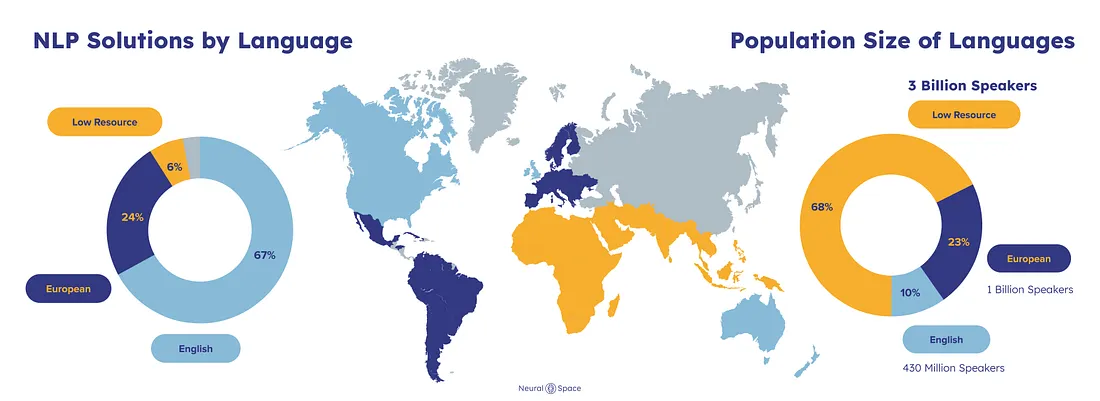
\includegraphics[width=0.85\textwidth]{Images/repartition.png}
    \caption[Répartition des langues selon leurs ressources en NLP]{Répartition des langues selon leur nombre de locuteurs et leurs ressources en NLP \cite{laumann2022challenges}}
    \label{fig:repartition-langues-nlp}
\end{figure}

%------------------------------------------------------------
\subsection{Défis du TAL pour les langues africaines}
%------------------------------------------------------------

\subsubsection{Manque de données linguistiques}

Le principal défi du \ac{TAL} pour les langues africaines réside dans le \textbf{manque de données linguistiques numériques} disponibles. La majorité des langues africaines disposent de très peu de corpus textuels, de ressources parallèles ou de bases lexicales exploitables, pour l'entraînement des modèles neuronaux \cite{ranathunga2023neural, agyei2024low}.

\subsubsection{Diversité dialectale}

Plusieurs langues africaines présentent une forte \textbf{diversité dialectale}. Une même langue peut posséder différentes variantes régionales, phonétiques ou lexicales, selon les communautés locutrices \cite{agyei2024low, mandiya2026lingala}.

Cette diversité complique la construction des corpus linguistiques et l'entraînement des modèles de \ac{TAL}, car les variations dialectales peuvent entraîner des incohérences dans les données \cite{haulai2023construction}.

\subsubsection{Absence de standardisation orthographique}

Certaines langues africaines ne disposent pas d'une orthographe totalement standardisée. Les variations d'écriture, les différences de transcription et les pratiques linguistiques locales peuvent produire plusieurs formes écrites pour un même mot \cite{haulai2023construction, jindal2017building}.

\subsubsection{Difficultés de collecte et d'annotation}

La collecte et l'annotation des données linguistiques nécessitent souvent un travail manuel important. Dans les \textbf{langues à faibles ressources}, les textes numériques sont rares et plusieurs contenus existent principalement sous forme orale ou papier \cite{agyei2024low, mandiya2026lingala}.

Ces difficultés rendent la constitution de corpus parallèles de qualité particulièrement laborieuse. Elles exigent le recours à des méthodes d'augmentation ou d'automatisation partielle de la collecte, afin de pallier le manque de données annotées \cite{ranathunga2023neural, sharma2023fully}.

%------------------------------------------------------------
\subsection{Présentation linguistique du ruund}
%------------------------------------------------------------

\subsubsection{Classification linguistique du ruund}

Le \textbf{ruund}, aussi appelé \textit{ruwund}, \textit{uruund} ou \textit{lunda du Nord} dans certaines classifications linguistiques, est une langue bantoue parlée par plus de 250 000 personnes, principalement en République Démocratique du Congo et en Angola. Il appartient à la famille des langues nigéro-congolaises et au groupe des langues bantoues \cite{frwiki:199251041}.

Cette langue est utilisée par une importante communauté locutrice, notamment dans la région du Katanga. Elle demeure néanmoins faiblement représentée dans les ressources numériques et les technologies linguistiques modernes \cite{frwiki:199251041}.

\subsubsection{Caractéristiques morphologiques}

Sur le plan morphologique, le ruund possède une structure fortement \textbf{agglutinante}, caractéristique des langues bantoues. L'organisation grammaticale de la langue repose principalement sur un système complexe de \textbf{classes nominales}, dans lequel les substantifs sont regroupés sous forme de classes singulier/pluriel ou de classes uniques. Chaque nom est généralement associé à un \textbf{préfixe nominal}, qui joue un rôle central dans les mécanismes d'accord grammatical \cite{kawasha2003lunda}.

Le système verbal du ruund présente également une morphologie riche et complexe. Le verbe est construit autour d'une \textbf{racine verbale}, combinée à plusieurs affixes flexionnels indiquant notamment l'accord du sujet, le temps, l'aspect, la négation ou encore la pronominalisation de l'objet. À cette structure s'ajoutent des extensions dérivationnelles telles que l'applicatif, le causatif ou le passif, capables de modifier la structure actancielle et la valeur sémantique du verbe \cite{kasombo2016structure, kawasha2003lunda}.

Par ailleurs, la morphotactique du ruund est soumise à des contraintes d'\textbf{harmonie vocalique}, entre la racine verbale et certains suffixes grammaticaux \cite{kasombo2016structure}. Cette richesse morphologique représente un défi important dans les tâches de traitement automatique des langues, notamment pour la tokenisation, la segmentation morphologique et la traduction automatique neuronale.

\subsubsection{Particularités syntaxiques et lexicales}

Le fonctionnement syntaxique du ruund repose sur un système de \textbf{concordance grammaticale} fortement développé. Les différents éléments associés au substantif, notamment les adjectifs, les démonstratifs, les possessifs ainsi que le verbe, s'accordent systématiquement avec le nom selon la classe nominale, le nombre et parfois la personne grammaticale \cite{kawasha2003lunda}.

L'identification des relations grammaticales telles que le sujet, l'objet direct ou l'objet indirect s'effectue à travers une combinaison de mécanismes. Ceux-ci incluent l'ordre des mots, la pronominalisation et certains marquages morphosyntaxiques \cite{kawasha2003lunda}.

Le ruund présente également des évolutions syntaxiques particulières, notamment l'apparition de constructions \textbf{passives impersonnelles} venant concurrencer certaines formes passives bantoues traditionnelles, construites à l'aide de suffixes verbaux. La langue se caractérise aussi par une diversité typologique importante des propositions relatives, ainsi que par différents mécanismes de détransitivation \cite{kawasha2003lunda}.

Sur le plan morphosyntaxique, plusieurs études soulignent également l'existence d'un certain \textbf{syncrétisme} entre les formes réflexives et réciproques. Elles relèvent aussi une convergence fonctionnelle entre les constructions passives et neutre-passives, malgré leurs différences structurelles \cite{kasombo2016structure, kawasha2003lunda}.

\subsubsection{Défis du ruund dans le NLP}

Le développement des applications \ac{NLP} pour le ruund fait face à plusieurs défis majeurs. La langue dispose de peu de corpus numériques, de ressources parallèles et d'outils linguistiques spécialisés. Les variations orthographiques et la rareté des données annotées compliquent également l'entraînement des modèles neuronaux.

Ces limitations réduisent les performances des systèmes de traduction automatique. Elles justifient la nécessité de développer des approches adaptées aux langues à faibles ressources, dans le contexte du ruund.

\subsection{Préservation linguistique et intelligence artificielle}

\subsubsection{Numérisation des langues africaines}

La numérisation des langues africaines constitue une étape essentielle pour leur intégration dans les technologies modernes de traitement automatique des langues. Ce processus consiste à transformer les ressources linguistiques disponibles sous forme orale ou papier, en données numériques exploitables par les systèmes informatiques \cite{agyei2024low, mandiya2026lingala}.

\subsubsection{IA et sauvegarde du patrimoine linguistique}

L'intelligence artificielle joue un rôle important dans la préservation du patrimoine linguistique. Les technologies de traitement automatique des langues permettent de documenter, d'analyser et de valoriser les langues peu représentées numériquement \cite{ranathunga2023neural, agyei2025dynamic}.

\subsubsection{Importance des ressources numériques locales}

Le développement de ressources numériques locales représente un enjeu vital pour les langues africaines, afin de surmonter la \textbf{« pénurie de données »} (\textit{data scarcity}) qui marginalise la majorité des langues mondiales \cite{ranathunga2023neural}. Pour le \textbf{ruund}, cette démarche s'appuie sur les avancées méthodologiques observées pour d'autres langues à faibles ressources, telles que le \textbf{mizo} \cite{haulai2023construction, lalrempuii2021improved}, le \textbf{pendjabi} \cite{jindal2017building} ou le \textbf{twi} \cite{agyei2024low}. Ces langues souffrent également d'un manque initial de présence numérique native. À l'instar du \textbf{mon} \cite{tun2025exploring}, l'absence de corpus parallèles structurés constitue un frein majeur au développement d'applications performantes. Elle rend indispensable la création d'outils linguistiques et de données annotées, pour renforcer les capacités des modèles neuronaux.

En s'appuyant sur les efforts de documentation menés pour le \textbf{quechua} \cite{sullatores2024desarrollo} ou l'\textbf{araméen} \cite{liebeskind2024machine}, la constitution de ressources pour le ruund s'inscrit dans une quête de \textbf{justice numérique}, visant à réduire la fracture technologique \cite{ranathunga2023neural, agyei2024low}. Cette production de données locales dépasse le simple cadre du progrès technique. Elle contribue aussi à préserver et à valoriser un patrimoine linguistique et culturel propre, face aux défis de la mondialisation, et permet à ses locuteurs de participer pleinement à l'écosystème numérique mondial.


%------------------------------------------------------------
\section{Analyse des travaux existants}
%------------------------------------------------------------




\subsection{Évolution des approches de traduction automatique}

\subsubsection{Approches symboliques}

Les premières tentatives de traduction automatique, dites \textbf{\ac{RBMT}}, reposaient sur des règles linguistiques et des dictionnaires bilingues élaborés manuellement par des experts. Elles s'avéraient précises pour des domaines restreints, mais coûteuses, difficiles à généraliser et incapables de gérer l'ambiguïté naturelle des langues complexes \cite{ranathunga2023neural, gangar2021hindi}.

\subsubsection{Approches statistiques}

La \textbf{traduction automatique statistique} (\ac{SMT}) a marqué un tournant, en apprenant des probabilités de traduction à partir de grands corpus parallèles. Les modèles de type \ac{PBSMT} peinent cependant à capturer les dépendances à longue distance et les structures syntaxiques divergentes, en particulier dans les langues morphologiquement riches \cite{lalrempuii2021improved, chanambam2022}.

\subsubsection{Approches neuronales modernes}

L'émergence de la \ac{TAN}, et plus particulièrement de l'architecture \textbf{Transformer}, a révolutionné le domaine en traitant les phrases de manière globale, via des mécanismes d'auto-attention. Ces modèles surpassent désormais les approches statistiques, en termes de fluidité et de cohérence contextuelle \cite{vaswani2017attention, ranathunga2023neural}.

%------------------------------------------------------------
\subsection{Travaux sur les langues à faibles ressources}
%------------------------------------------------------------

\subsubsection{Traduction neuronale multilingue}

La traduction multilingue (\ac{MNMT}) permet de mutualiser les connaissances entre plusieurs langues au sein d'un modèle unique. Cette approche est cruciale pour les langues peu dotées, car elle facilite le transfert de connaissances depuis des langues à fortes ressources vers des langues cibles \cite{ali2026hybrid, baladaspanda2023improving}. La qualité du transfert dépend également du choix de la stratégie de segmentation en sous-mots et de la nature du transfert cross-lingual entre les langues concernées \cite{meyer2024systematic, toraman2022impact}.

\subsubsection{Fine-tuning pour les langues sous-représentées}

L'adaptation de modèles pré-entraînés comme \textbf{mBART-50} ou \textbf{NLLB-200} via le \textit{fine-tuning} est la stratégie la plus efficace pour les petits jeux de données. Un modèle pré-entraîné fournit en effet une excellente initialisation grammaticale, même avec un corpus restreint \cite{kozhirbayev2024enhancing, hong2024cantonmt}. Cette approche a également démontré son efficacité dans des contextes de traduction entre langues asiatiques à faibles ressources \cite{tran2024improving}.

\subsubsection{Traduction basée sur des corpus bibliques et textes poétiques}

La Bible est souvent l'une des seules ressources parallèles disponibles pour de nombreuses langues à faibles ressources (mizo, twi, quechua). Elle offre un alignement précis par versets. Son domaine reste toutefois restreint, ce qui limite souvent la capacité de généralisation du modèle final \cite{chanambam2022, angel2023comparing}.

La poésie présente des défis uniques en \ac{TAN}, notamment la préservation des patterns de rimes et de la structure métrique. Les travaux existants indiquent que les modèles neuronaux, bien que performants, peinent encore à restituer la créativité littéraire sans un ajustement spécifique \cite{dundjer2020automatic, liebeskind2024machine}.

\subsubsection{Travaux sur les langues africaines et bantoues}

Les langues bantoues, comme le ruund, font face à des défis majeurs en matière de traitement de l'information et de développement informatique. Ces difficultés structurelles, combinées au manque de ressources numériques, soulignent l'importance de construire des ressources locales pour les langues africaines, souvent exclues des technologies numériques \cite{ranathunga2023neural}.

%------------------------------------------------------------
\subsection{Analyse critique des travaux existants}
%------------------------------------------------------------

\subsubsection{Forces des approches actuelles}

Les modèles basés sur les \textbf{Transformers} et l'apprentissage par transfert permettent d'obtenir des résultats exploitables, là où les méthodes traditionnelles échouaient. Cette supériorité empirique a été démontrée pour plusieurs paires de langues à faibles ressources, notamment le mizo--anglais \cite{lalrempuii2021improved} et le môn--anglais \cite{tun2025exploring}.

\subsubsection{Limites liées aux données}

La \ac{TAN} est extrêmement gourmande en données. Les performances chutent drastiquement en dessous de 10~000 paires de phrases \cite{ranathunga2023neural}. Notre corpus de 8~431 paires se situe précisément dans cette zone critique, ce qui rend l'usage du transfert d'apprentissage indispensable \cite{ma2025dongba}.

\subsubsection{Difficultés liées aux langues bantoues}

Le manque de standardisation orthographique et la richesse des affixes verbaux compliquent la tâche de tokenisation. Les modèles généralistes peinent souvent à capturer l'harmonie vocalique et les spécificités tonales, sans données massives.

\subsubsection{Limites des métriques d'évaluation}

Le score \ac{BLEU}, bien que standard, ne corrèle pas toujours parfaitement avec le jugement humain, pour les langues à faibles ressources \cite{lankford2022human, lalrempuii2021improved}. Notre choix d'inclure une évaluation humaine est donc scientifiquement justifié, pour valider l'adéquation sémantique \cite{tun2025exploring}.

\subsubsection{Synthèse comparative des travaux}

Le Tableau~\ref{tab:synthese_travaux} présente une analyse comparative de seize études représentatives, portant sur la traduction automatique pour les langues à faibles ressources. Il synthétise les approches méthodologiques, les performances obtenues, la complexité des systèmes, leur robustesse ainsi que leurs limites principales.

\begingroup
\renewcommand{\arraystretch}{1.4}
\small
\rowcolors{2}{gray!10}{white}
\begin{longtable}{p{2.8cm}p{2.8cm}p{2.2cm}p{1.9cm}p{1.9cm}p{3.2cm}}
\toprule
\textbf{Auteur(s)} & \textbf{Approche} & \textbf{Performance} & \textbf{Complexité} & \textbf{Robustesse} & \textbf{Limites principales} \\
\midrule
\endfirsthead
\endhead

\bottomrule
\endfoot

\bottomrule
\endlastfoot
\citeauthor{ali2026hybrid} \cite{ali2026hybrid} &
\ac{MNMT} non supervisée (XLM-R + ACL) &
+1.2 \ac{BLEU} (bilingue) &
Élevée &
Haute &
Qualité médiocre sur phrases longues ; dépendance aux dictionnaires bilingues \\
\citeauthor{lalrempuii2021improved} \cite{lalrempuii2021improved} &
Comparaison SMT vs NMT (mizo) &
Transformer $\gg$ LSTM et SMT &
Modérée &
Moyenne &
Baisse radicale sur phrases longues ; manque de ressources pour le mizo \\
\citeauthor{kozhirbayev2024enhancing} \cite{kozhirbayev2024enhancing} &
Fine-tuning mBART-50 &
+11.95 \ac{BLEU} (kazakh--russe) &
Moyenne &
Haute &
Sensibilité à la qualité des données de fine-tuning et aux hyperparamètres \\
\citeauthor{ahmadnia2021impact} \cite{ahmadnia2021impact} &
Filtrage de données pseudo-parallèles &
BLEU $>$ baselines non filtrées &
Modérée &
Améliorée &
Corpus filtré très réduit ; généralisation limitée \\
\citeauthor{dai2025tfttl} \cite{dai2025tfttl} &
Transfert TFT-TL (niveau token) &
19.88 \ac{BLEU} (Tr--En) &
Élevée &
Excellente &
Instabilité possible à certaines étapes d'apprentissage \\
\citeauthor{brahma2023selectnoise} \cite{brahma2023selectnoise} &
SELECTNOISE (injection de bruit) &
Surpasse les baselines zero-shot &
Élevée &
Robuste &
Efficacité réduite si les scripts des langues sont trop différents \\
\citeauthor{chen-fazio-2021-morphologically} \cite{chen-fazio-2021-morphologically} &
Segmentation morphologique (PRPE) &
23.4 \ac{BLEU} (quechua) &
Modérée &
Bonne &
Nécessite une liste d'affixes préalable (connaissances linguistiques) \\
\citeauthor{bala2024multilingual} \cite{bala2024multilingual} &
MNMT + translittération (Indic--Indic) &
+6.74 \ac{BLEU} (malayalam) &
Modérée &
Bonne &
Interférence négative sur certains groupes linguistiques rares \\
\citeauthor{tun2025exploring} \cite{tun2025exploring} &
Hybride SMT, NMT, BART fine-tuné &
BART + \ac{SentencePiece} = meilleurs résultats &
Élevée &
Bonne &
Complexité morphologique du môn non résolue par le seul transfert \\
\citeauthor{ahmed2023guit} \cite{ahmed2023guit} &
Rétro-traduction itérative (mizo) &
+3.65 \ac{BLEU} par itération &
Modérée &
Moyenne &
Inefficace sur phrases très longues \\
\citeauthor{gronroos2020transfer} \cite{gronroos2020transfer} &
Multi-task learning programmé &
+12.7 \ac{BLEU} via \ac{MNMT} + rétro-traduction &
Élevée &
Haute &
Rendements décroissants au-delà de 10~000 phrases \\
\citeauthor{aci2025morphological} \cite{aci2025morphological} &
Analyse de profondeur (anglais--turc) &
47.85 \ac{BLEU} (Transformer 3 couches) &
Élevée &
Excellente &
Chute de performance si la profondeur dépasse le seuil optimal \\
\citeauthor{kann2022americasnli} \cite{kann2022americasnli} &
AmericasNLI (langues indigènes) &
+24.53\% pour le quechua &
Haute &
Moyenne &
Répétition de sous-mots dans les sorties ; sensibilité au domaine \\
\citeauthor{goyal2020efficient} \cite{goyal2020efficient} &
Translittération unifiée (indo-aryen) &
+5 points \ac{BLEU} en moyenne &
Modérée &
Bonne &
Ambiguïtés à l'inférence entre langues proches \\
\citeauthor{hong2024cantonmt} \cite{hong2024cantonmt} &
CANTONMT (rétro-traduction + commutation) &
SacreBLEU 16.8 &
Haute &
Moyenne &
Corpus très réduit (60k) par rapport à la population cible (80M locuteurs) \\
\citeauthor{rani2023filtering} \cite{rani2023filtering} &
Filtrage cross-validation (sanskrit--hindi) &
+1.85 \ac{BLEU} (token-level) &
Modérée &
Bonne &
Corpus filtré final très réduit (300 paires test) ; portée statistique limitée \\
\end{longtable}
\addtocounter{table}{-1}
{\captionsetup{hypcap=false}
\captionof{table}{Synthèse comparative des travaux existants sur la TAN pour les langues à faibles ressources}
\label{tab:synthese_travaux}}
\endgroup


%------------------------------------------------------------
\subsection{Gap scientifique et positionnement du mémoire}
%------------------------------------------------------------

\subsubsection{Absence de \ac{TAN} sur le ruund}

Il n'existe actuellement aucun système de traduction automatique robuste documenté pour le ruund. Ce travail comble un vide numérique pour cette communauté linguistique.

\subsubsection{Insuffisance des ressources numériques ruund--français}

Les sources disponibles pour le ruund sont fragmentaires et non structurées pour le \ac{ML}. L'effort de \textit{Data Engineering} réalisé dans ce travail, à savoir le nettoyage, la normalisation et l'alignement de 8~431 paires, constitue une contribution majeure à la documentation numérique de cette langue \cite{Mununga2026openruund}.

\subsubsection{Justification scientifique du mémoire}

Ce mémoire se positionne à la pointe de la recherche actuelle. Il utilise le \textit{fine-tuning} de modèles étatiques (NLLB-200, mBART-50) pour compenser la rareté des données, selon une démarche validée pour d'autres langues à faibles ressources telles que le môn \cite{tun2025exploring}.

\subsubsection{Contribution attendue de la recherche}

Outre le système de traduction, ce travail propose une méthodologie pour construire des jeux de données exploitables à partir de sources religieuses et poétiques. Cette méthodologie ouvre la voie à une future généralisation vers des domaines variés.

\section*{Conclusion partielle}

L'analyse de la littérature met en évidence le manque de ressources numériques pour les langues à faibles ressources. Elle souligne aussi l'intérêt des corpus parallèles et des modèles multilingues pré-entraînés pour améliorer la traduction automatique. Ces constats justifient la présente recherche sur le ruund, langue encore peu documentée dans les technologies du langage \cite{ranathunga2023neural, haulai2023construction, kozhirbayev2024enhancing}.

Le chapitre suivant présente la construction du corpus parallèle ruund--français, depuis la collecte des données jusqu'à leur alignement et leur validation.